\chapter{Feature Selection}
\label{chapter:analysis}

\section{Sentinel-2 Seasons}
\label{section:seasonal}

Fig.\,\ref{fig:seasonal_selection} shows the performance of the CNN model across different seasons, with metrics including recall, precision, weighted f1-score, precision-recall curve area under the curve (PRC), and receiver operating characteristic area under the curve (AUC). Filled boxes indicate the combination of seasons used to train and validate the model. Blue boxes indicate a combination of 3D CNN and fully-connected layers and the orange box indicates the use of a similar model but with the introduction Long Short-Term Memory (LSTM) alongside 3D convolutions and fully-connected layers.

\begin{figure}[ht]
    \centering
    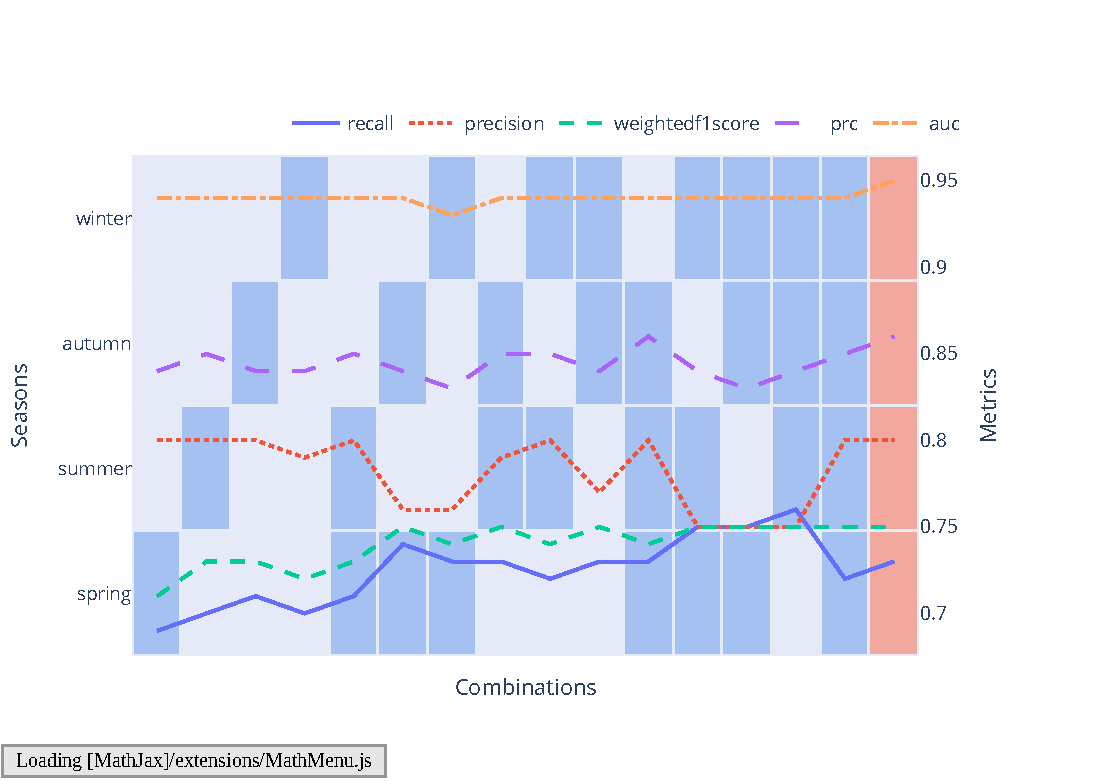
\includegraphics[width=0.98\linewidth, trim={20pt 40pt 10pt 30pt}, clip]{figures/figures_analysis/seasonal_selection.pdf}
    \caption{Seasonal Sentinel-2 analysis for all season combinations using a 3D CNN.}
    \label{fig:seasonal_selection}
\end{figure}

3D convolutions were selected for this model due to their suitability for this problem as they can effectively capture the spatial and spectral dependencies in the multi-temporal Sentinel-2 data. By considering the additional temporal dimension, 3D convolutions can leverage seasonal variations and changes in vegetation phenology, which are crucial for accurate tree genus classification.

LSTM was introduced to the model alongside 2D convolutions because they process the spatial structure of the Sentinel-2 images through convolution operations while simultaneously capturing temporal sequences. This dual capability allows the model to learn intricate spatial patterns within each image and understand how these patterns evolve over time.

The selected metrics used to create Fig.\,\ref{fig:seasonal_selection} are tailored to address class imbalance. Recall measures the ability to capture instances of minority classes, while precision assesses the accuracy of positive predictions. The weighted f1-score combines precision and recall, considering class support. PRC emphasizes the precision-recall trade-off, particularly for minority classes. AUC evaluates overall model performance across all thresholds, indicating its discriminative ability.

For individual seasons, the model performs best in summer and autumn overall across the metrics. This suggests that the CNN model is more effective at classifying tree genera during these times, likely due to clearer and more distinct spectral signatures in the data collected during summer and autumn. The lower performance in spring and winter might be attributed to less distinct spectral signatures or more challenging environmental conditions, such as cloud cover and snow, which can affect data quality.

Based on the weighted f1-scores shown in Fig.\,\ref{fig:seasonal_selection}, adding more seasons does not seem to offer significant benefits. For instance, some two-season combinations, such as summer and autumn, performed on par with the more complex four-season models. Additionally, single-season models were only a few percentage points below the top-performing models.

Based on these results, further analysis focused solely on summer seasons. This approach benefits from faster model training and reduced storage requirements, as adding an extra season nearly doubles the storage needs, a challenge that intensifies with the extension of the analysis over additional years. Despite these adjustments, a complete Sentinel-2 dataset for a single season still requires nearly 200\,GB, or approximately 1\,MB per location.

\section{Sentinel-2 Bands}

\begin{figure}[ht]
    \centering
    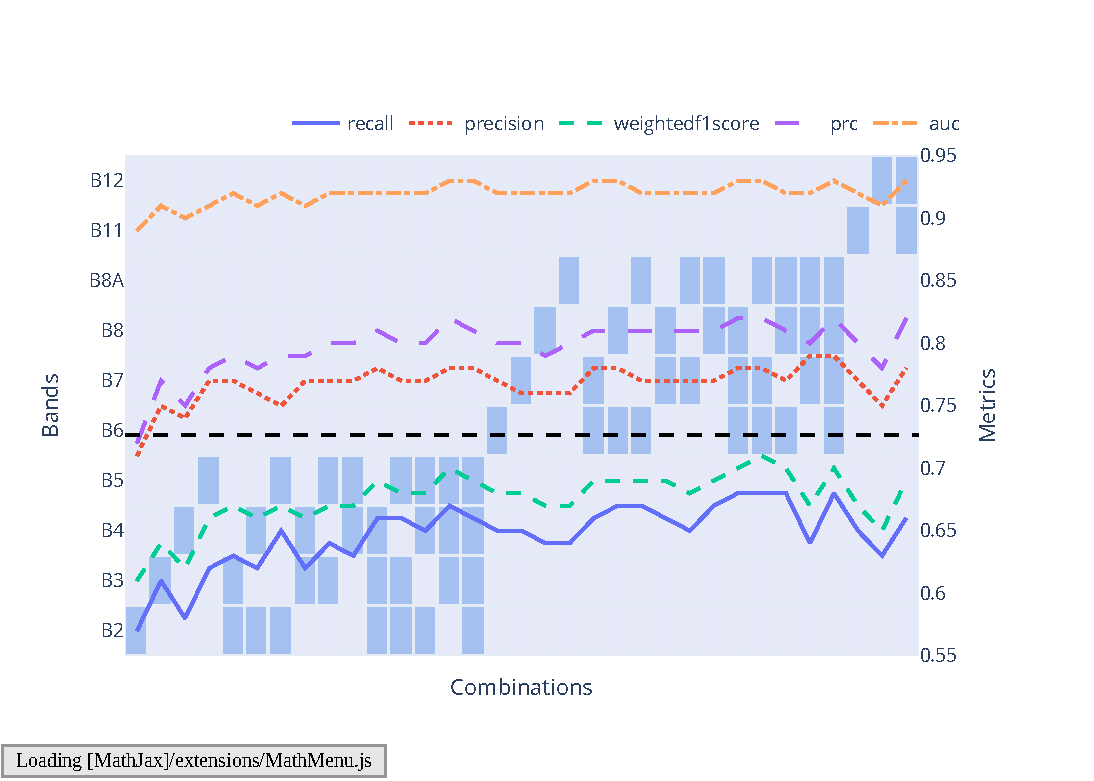
\includegraphics[width=0.98\linewidth, trim={20pt 40pt 10pt 30pt}, clip]{figures/figures_analysis/band_selection.pdf}
    \caption{Sentinel-2 analysis for all combinations within three band groups using a CNN. The horizontal black line represents the weighted f1-score for all bands.}
    \label{fig:band_selection}
\end{figure}

In addition to the seasonal analysis in Section\,\ref{section:seasonal}, another analysis was conducted to identify the most effective band combinations. Due to the large number of possible combinations, a direct analysis was impractical. Instead, Sentinel-2 bands were divided into three groups based on summer correlation groupings shown in Fig.\,\ref{fig:season_correlation}: B2, B3, B4, and B5; B6, B7, B8, and B8A; and B11 and B12. 

The resulting analysis, shown in Fig.\,\ref{fig:band_selection}, indicates that NIR and SWIR bands perform slightly better overall. Based on these results, another group was selected: B2, B3, B6, B8, and B11. These bands represented the best combinations that resulted in a practical analysis within the available timeframe.

\begin{figure}[ht]
    \centering
    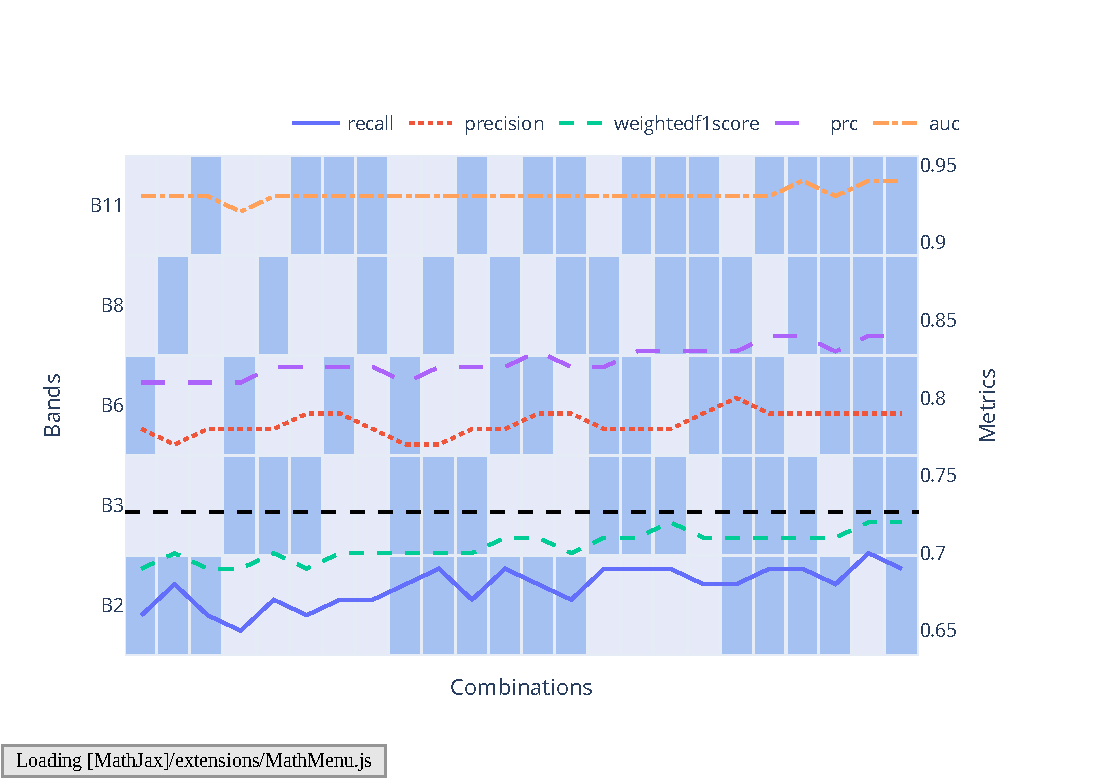
\includegraphics[width=0.98\linewidth, trim={20pt 40pt 10pt 30pt}, clip]{figures/figures_analysis/band_selection_further.pdf}
    \caption{Sentinel-2 analysis for selected combinations between each of the three groups using a CNN. The horizontal black line represents the weighted f1-score for all bands.}
    \label{fig:band_selection_further}
\end{figure}

Fig.\,\ref{fig:band_selection_further} shows that most selected combinations performed relatively well, as indicated by their proximity to the weighted f1-score for all bands. Based on these results, the most reasonable choices appear to be B3, B8, and B11, or the same but with B6 in addition. As the B6 combination displays better recall, precision, and weighted f1-score, as well as taking a fraction of storage compared to 10\,m bands due to being 20\,m. For the 250,000 samples, this combination should take roughly 50 GB of storage. As such, the combination B3, B6, B8, and B11, was used for the remainder of this study.

\section{Soil and Elevation}

\begin{figure}[ht]
    \centering
    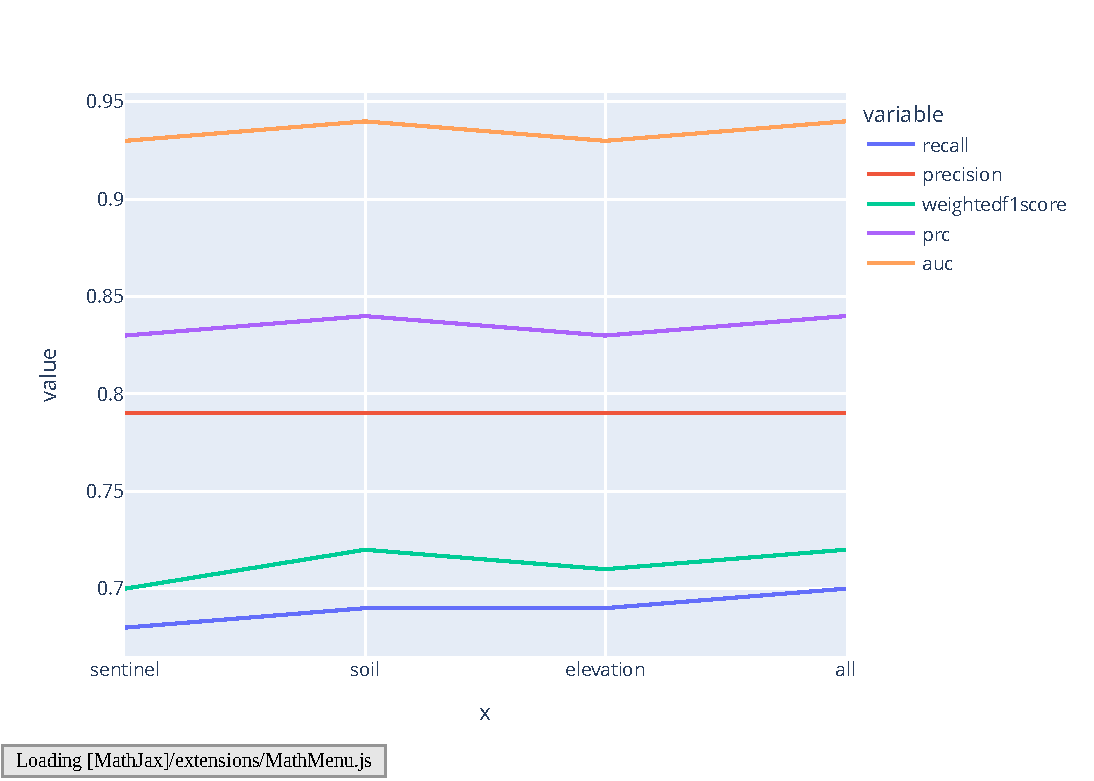
\includegraphics[width=0.98\linewidth, trim={20pt 40pt 10pt 30pt}, clip]{figures/figures_analysis/soil_elevation_analysis.pdf}
    \caption{Analysis of SoilGrids and elevation data integration.}
    \label{fig:soil_elevation_analysis}
\end{figure}

Fig.\,\ref{fig:soil_elevation_analysis} demonstrates the performance metrics for different combinations of Sentinel-2, SoilGrids, and elevation data in tree genus classification. Sentinel-2 data alone provides a solid baseline, attributed to its high resolution and rich spectral information. When considering SoilGrids data alone, the metrics are lower than those for Sentinel-2, reflecting the coarse resolution and potentially limited predictive power for this specific task. Similarly, elevation data alone shows lower performance metrics, indicating that while elevation is a relevant feature, it does not provide sufficient information by itself for accurate classification of tree genera. The combined use of these datasets shows marginal improvements, suggesting that while additional data may contribute some value, Sentinel-2's high-resolution spectral data is the most significant factor in the model's performance.

Given that Sentinel-2 data alone provides strong results, further enhancements and optimizations were solely focused on this dataset. 

\section{Summary}

The analysis highlights the influence of various seasonal combinations, Sentinel-2 bands, and additional datasets such as soil composition and elevation data on the performance of the CNN model for tree genus classification. Summer and autumn seasons were found to be the most effective for accurate classification, with minimal gains observed from including additional seasons. In terms of band selection, NIR and SWIR bands demonstrated the best results, leading to the selection of the B3, B6, B8, and B11 combination for further analysis due to its optimal balance between performance and storage efficiency. While soil composition and elevation data provided marginal improvements, Sentinel-2 data remained the most critical factor in model accuracy. Consequently, further optimizations focused primarily on the B3, B6, B8, and B11 bands of Sentinel-2.